%% public_data_sources.tex
%% Copyright: James Hutton Institute 2016
%% Author: Leighton Pritchard
%% Public Data Sources

% NCBI
\begin{frame}
  \frametitle{NCBI \hfill 
\includegraphics[height=0.1\textheight,valign=t]{images/NCBI}}
    \begin{alertblock}{\href{http://www.ncbi.nlm.nih.gov/}{http://www.ncbi.nlm.nih.gov/}}
      Repository of record for pathogen (and other) genome data
    \end{alertblock}
    \begin{itemize}
      \item Example: \textcolor{hutton_purple}{\href{http://www.ncbi.nlm.nih.gov/genome/490}{\textit{Ralstonia solanacearum}}}
        \begin{itemize}
          \item Browser interface
          \item FTP repositories of genome data \\
            - \textcolor{hutton_purple}{\href{http://ftp.ncbi.nlm.nih.gov/genomes/refseq/bacteria/Ralstonia_solanacearum/latest_assembly_versions/}{RefSeq}} \\
            - \textcolor{hutton_purple}{\href{http://ftp.ncbi.nlm.nih.gov/genomes/genbank/bacteria/Ralstonia_solanacearum/latest_assembly_versions/}{GenBank}}
        \end{itemize}
    \end{itemize}
    \begin{center}
      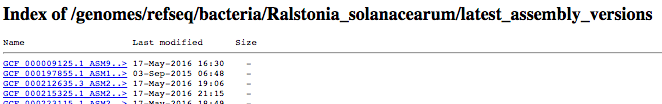
\includegraphics[width=0.75\textwidth]{images/refseq_list} \\ 
      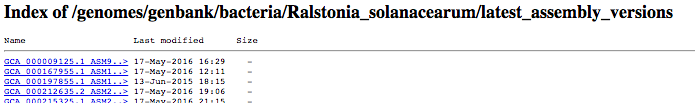
\includegraphics[width=0.75\textwidth]{images/genbank_list}      
    \end{center}    
\end{frame}

% GENBANK VS REFSEQ
\begin{frame}
  \frametitle{GenBank \textit{vs} RefSeq}
    \begin{alertblock}{\href{http://www.ncbi.nlm.nih.gov/genbank/}{GenBank}}
      \begin{itemize}
        \item part of \textcolor{hutton_purple}{\href{http://www.insdc.org/}{International Nucleotide Sequence Database Collaboration (INSDC)}}: EMBL/NCBI/DDBJ
        \item records 'owned' by submitter
        \item may include redundant information
      \end{itemize}
    \end{alertblock}
    \begin{block}{\href{http://www.ncbi.nlm.nih.gov/refseq/about}{RefSeq}}
      \begin{itemize}
        \item not part of INSDC
        \item records derived from GenBank, 'owned' by NCBI
        \item stable non-redundant foundation for functional and diversity studies
      \end{itemize}
    \end{block}
\end{frame}

% ENSEMBL
\begin{frame}
  \frametitle{Ensembl \hfill 
\includegraphics[height=0.1\textheight,valign=t]{images/ensembl_metazoa_logo}}
    \begin{alertblock}{\href{http://www.ensembl.org}{http://www.ensembl.org}}
      Automated annotation on selected genomes
    \end{alertblock}
    \begin{itemize}
      \item \textcolor{hutton_green}{\textbf{Specialised sub-collections}}
      \begin{itemize}
        \item Ensembl Protists: \textcolor{hutton_purple}{\href{http://protists.ensembl.org/}{http://protists.ensembl.org/}}
        \item Ensembl Bacteria: \textcolor{hutton_purple}{\href{http://bacteria.ensembl.org/}{http://bacteria.ensembl.org/}}
        \item Ensembl Fungi: \textcolor{hutton_purple}{\href{http://fungi.ensembl.org/}{http://fungi.ensembl.org/}}
      \end{itemize}
      \item \textcolor{hutton_blue}{\textbf{Downloadable resources}}
      \begin{itemize}
        \item e.g. \textcolor{hutton_purple}{\href{http://ftp.ensemblgenomes.org/pub/protists/}{ftp://ftp.ensemblgenomes.org/pub/protists/}}
      \end{itemize}
      \item \textcolor{RawSienna}{\textbf{Ready-made comparative genomics!}}
      \begin{itemize}
        \item \textcolor{hutton_purple}{\href{http://protists.ensembl.org/Phytophthora_infestans/Location/Compara_Alignments/Image?align=119329;db=core;r=supercont1.34:559462-573700}{\textit{Phytophthora} genomics alignments (Avr3a)}}
        \item \textcolor{hutton_purple}{\href{http://protists.ensembl.org/Phytophthora_infestans/Gene/Compara_Tree/pan_compara?db=core;g=PITG_14371;r=supercont1.34:559462-573700;t=PITG_14371T0}{Gene trees (Avr3a)}}
      \end{itemize}
    \end{itemize}
\end{frame}

% OTHER SOURCES
\begin{frame}
  \frametitle{Other Sources}
    \begin{itemize}
      \item \textcolor{hutton_green}{\textbf{Sequencing centres, e.g.}}
      \begin{itemize}
        \item \textcolor{hutton_purple}{\href{http://genome.jgi.doe.gov/}{JGI Genome Portals}}
        \item Ensembl Bacteria: \textcolor{hutton_purple}{\href{https://www.broadinstitute.org/}{Broad Institute}} - now retiring their online resources
      \end{itemize}
      \item \textcolor{hutton_blue}{\textbf{Specialist databases, e.g.}}
      \begin{itemize}
        \item \textcolor{hutton_purple}{\href{http://fungidb.org/fungidb/}{FungiDB}} - fungi and oomycetes
        \item \textcolor{hutton_purple}{\href{http://cpgr.plantbiology.msu.edu/}{CPGR}} - fungi and oomycetes (not recently updated)
      \end{itemize}
      \item \textcolor{RawSienna}{\textbf{Your friendly local sequencing centre!}}
      \begin{itemize}
        \item \textcolor{hutton_purple}{\href{http://asperasoft.com/}{Aspera}} is commonly used to connect to your private data
      \end{itemize}
    \end{itemize}
\end{frame}

% OPTIONAL WORKSHEET
\begin{frame}
  \frametitle{Optional Worksheet}
  \begin{alertblock}{\url{worksheets/01-downloading_data_biopython.ipynb}}
    Downloading genome data from NCBI with Biopython
  \end{alertblock}
  \begin{itemize}
    \item \textcolor{hutton_purple}{\href{http://mybinder.org/repo/widdowquinn/Teaching-EMBL-Plant-Path-Genomics}{MyBinder link}}
  \end{itemize}
\end{frame}